% ***************************************************
% Appendix
% ***************************************************
\chapter{Supplementary information for Chapter 5}

\hypertarget{pama-nyungan-reference-phylogeny}{%
\subsection{Pama-Nyungan reference
phylogeny}\label{pama-nyungan-reference-phylogeny}}

Quantifying phylogenetic signal requires an independently-derived
reference phylogeny as a yardstick. Our reference phylogeny is a 285-tip
Pama-Nyungan phylogeny inferred by the second author. Figure S1 gives a
111-tip subset of this phylogeny, corresponding to the 111 doculects
used in this study.

\begin{figure}
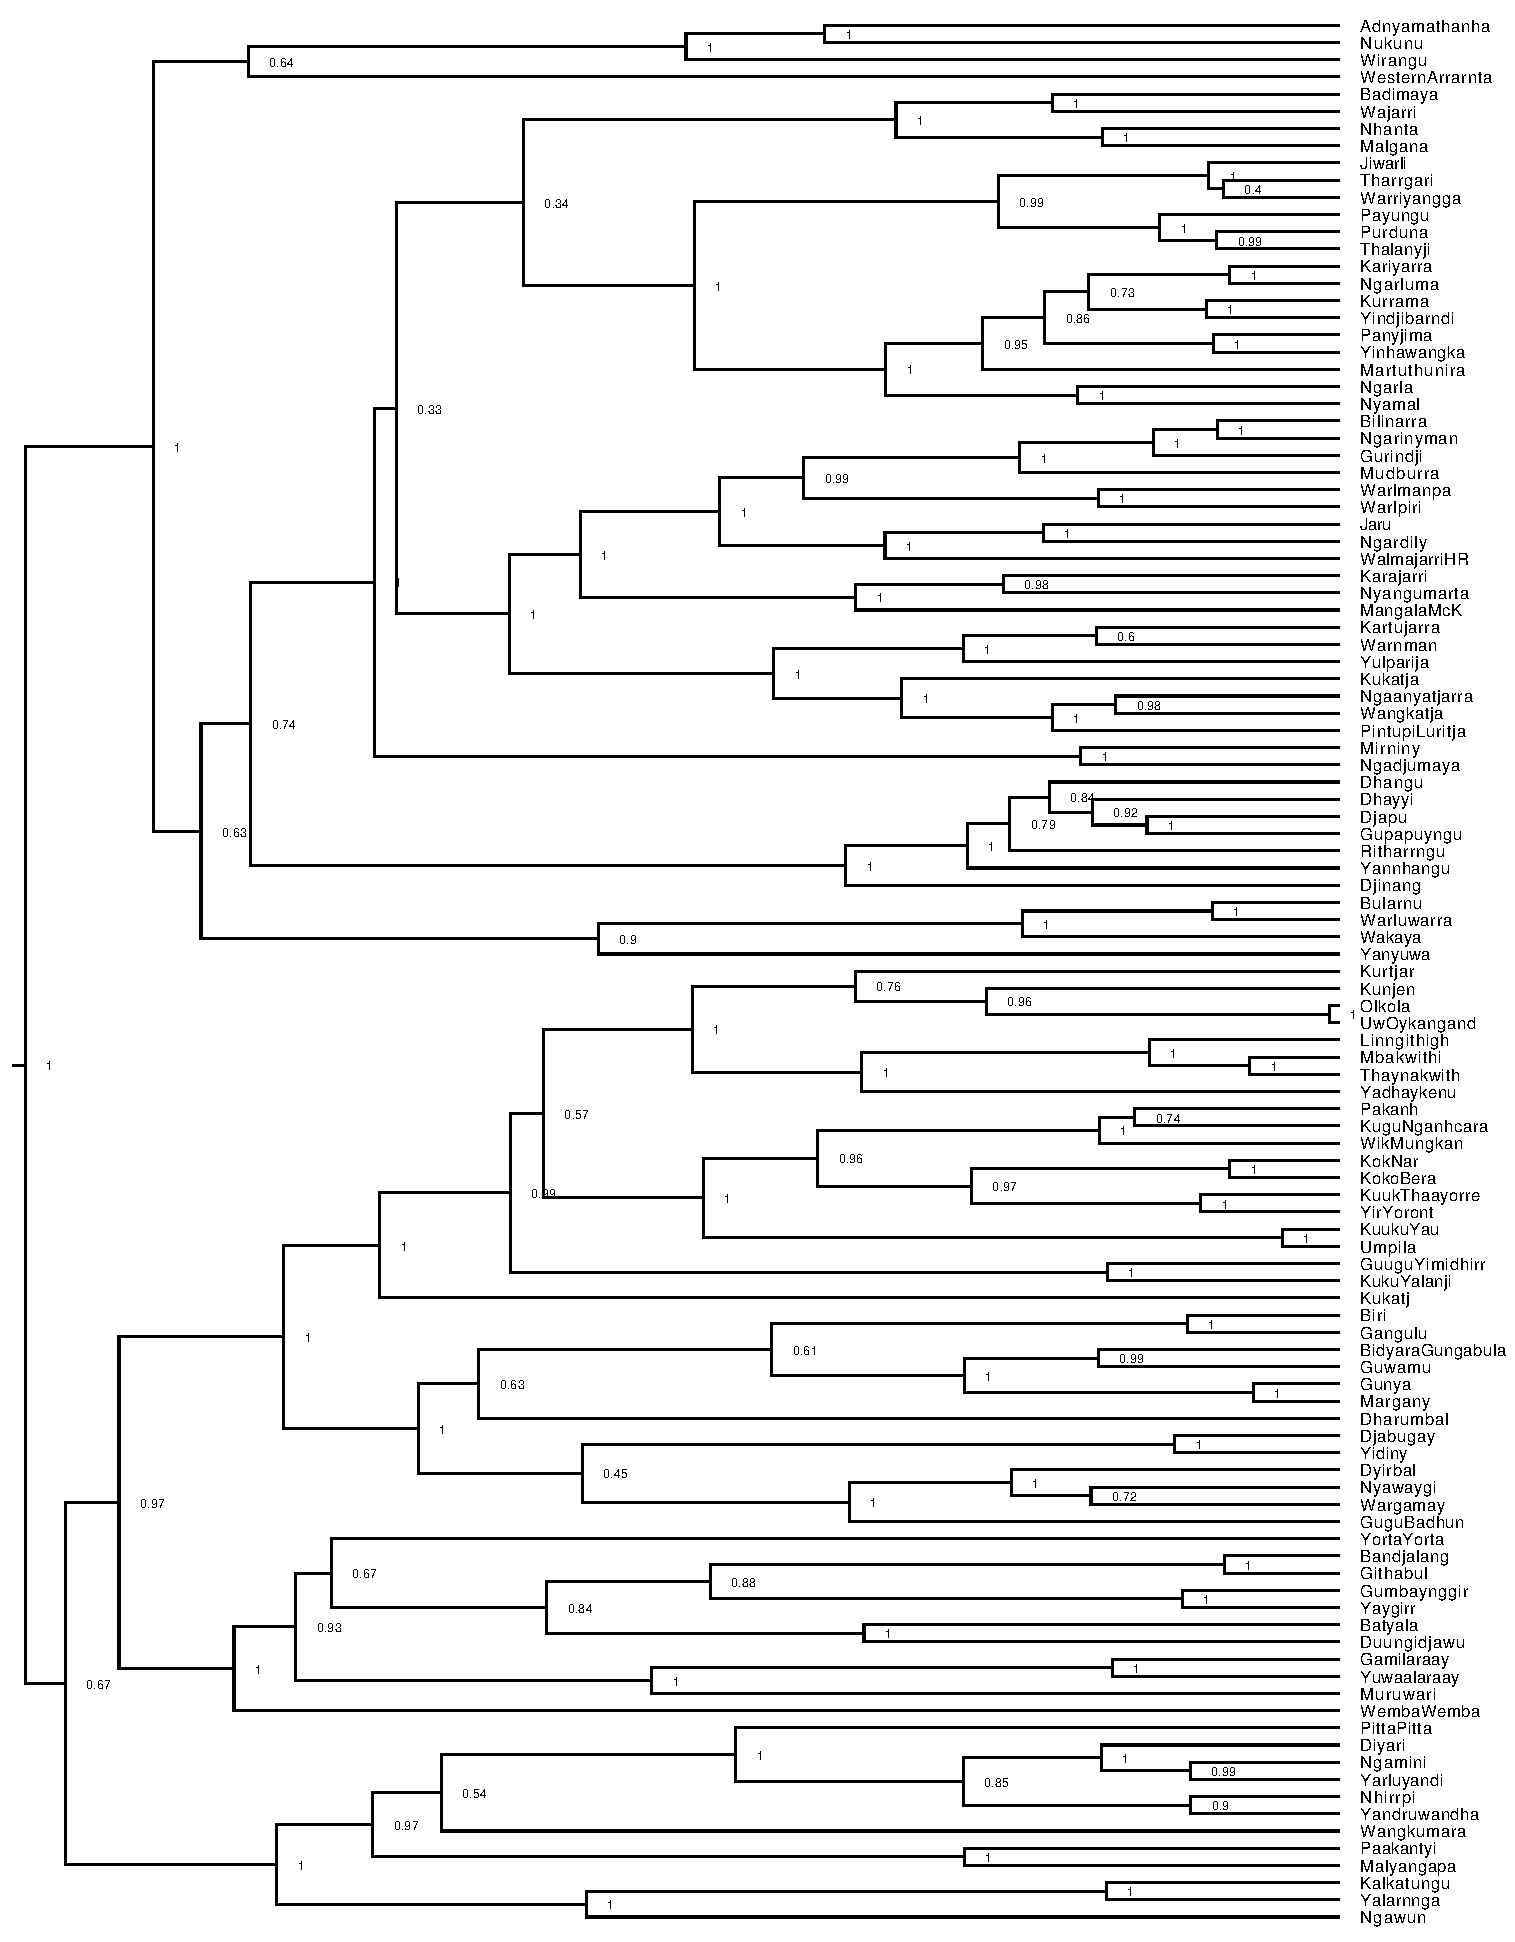
\includegraphics[width=1\linewidth]{Appendix-B/fig/PN_beast_pruned} \caption{Pama-Nyungan reference phylogeny. Node labels are posterior probabilities, giving an indication of support for each node. Although there is no strict, conventional cut-off, clades with posterior values above 0.5 are considered supported and values above 0.8 are considered strongly supported (Bowern \& Atkinson 2012, p.829).}\label{fig:plot-ref-tree2}
\end{figure}

As discussed in the main paper, the reference phylogeny was constructed
using Bayesian phylogenetic methods in the software BEAST2
\autocite{bouckaert_beast_2014}. Bayesian phylogenetic methods use a
Markov Chain Monte Carlo (MCMC) procedure to efficiently search the
hypothesis space of possible trees and return a large posterior sample
of similarly credible alternatives (capturing phylogenetic uncertainty).
The tree in Figure S1 above is a maximum clade credibility tree, which
is a summation of the posterior sample where the likelihood of all nodes
in the tree (in terms of how frequently a given node reappears across
the posterior sample) is maximized.

For further details on the Pama-Nyungan phylogeny used as a reference
phylogeny in this study, see \textcite{bowern_pama-nyungan_2015}. See
also \textcite{bowern_computational_2012}, which infers a Pama-Nyungan
phylogeny in the same way, using exactly the same evolutionary model
parameters, but with an earlier iteration of the dataset containing
fewer doculects. Additional discussion of the general process of
constructing language phylogenies in BEAST2 can be found in
\textcite{bouckaert_origin_2018}, although a different evolutionary
model is used.

The reference phylogeny was inferred using lexical cognate data, coded
according to the principles of the Comparative Method. The cognate data
used in the reference phylogeny is publicly available on Zenodo
\autocite{bowern_pama-nyungan_2018} and also as a subset of the
305-language dataset in \textcite{bouckaert_origin_2018}. This latter
source also includes a Perl script for converting multistate cognate
judgements into a binary matrix for use with BEAST2 phylogenetic
software and will include information on underlying sources.

\newpage

\hypertarget{phy-sig-wordlist-sources}{%
\subsection*{Wordlist sources}\label{phy-sig-wordlist-sources}}
\addcontentsline{toc}{subsection}{Wordlist sources}

The 111 wordlists used in this study are contained within the Ausphonlex
database, under development by \textcite{round_ausphon-lexicon_2017}.
All underlying wordlist data is available, either publicly in the
CHIRILA database \autocite{bowern_chirila_2016} or elsewhere in
published or archived form. A list of original sources for all wordlists
is presented below.

\textbf{Adnyamathanha}

CHIRILA source: CHIRILA/v2/McEnteeMcKenzie

\fullcite{mcentee_adna-mat-na_1992}

Phonemic normalization: Coda tap normalized as vibrant. Otherwise,
voiced stops, taps and fricatives normalized to lenis obstruents.

\textbf{Mbakwithi}

CHIRILA source: CHIRILA/v1/ASEDA0240

\fullcite{crowley_mbakwithi_1989}

\textbf{Badimaya}

\fullcite{marmion_badimaya_1995}

Phonemic normalization: Double a normalized to long vowel.

\textbf{Pakanh}

\fullcite{hamilton_pakanh_1997}

\textbf{BidyaraGungabula}

\fullcite{breen_bidyara_1973}

\textbf{Bilinarra}

\fullcite{meakins_bilinarra_2013}

\textbf{Biri}

CHIRILA source: CHIRILA/v1/Terrell

\fullcite{terrill_biri_1999}

\textbf{Bularnu}

\fullcite{breen_bularnu_1988}

\textbf{Batyala}

\fullcite{bell_sketch_2003}

\textbf{Dhangu}

\fullcite{zorc_yolngu_2004}

Phonemic normalization: Lenis retroflex stop normalized to retroflex
flap.

\textbf{Dharumbal}

CHIRILA source: CHIRILA/v2/ter02

\fullcite{terrill_dharumbal:_2002}

\textbf{Dhayyi}

\fullcite{wunungmurra_dhalwangu_1993}

Phonemic normalization: Lenis retroflex stop normalized to retroflex
flap; all other voicing is allophonic.

\textbf{Diyari}

\fullcite{austin_grammar_1981}

Phonemic normalization: Phonetic trill-released stop normalized as stop
+ trill. Otherwise, voiced stops normalized as taps.

\textbf{Djabugay}

\fullcite{robertson_jaabugay_1997}

\textbf{Djapu}

CHIRILA source: CHIRILA/v1/mor83

\fullcite{morphy_djapu_1983}

Phonemic normalization: Lenis retroflex stop normalized to retroflex
flap.

\textbf{Djinang}

CHIRILA source: CHIRILA/v1/ASEDA0009

\fullcite{waters_djinang_1988}

Phonemic normalization: Glottal closure normalized to a segment phoneme.

\textbf{Duungidjawu}

CHIRILA source: CHIRILA/v2/K\&W 04

\fullcite{kite_duungidjawu_2004}

\textbf{Dyirbal}

CHIRILA source: CHIRILA/v1/dix72

\fullcite{dixon_dyirbal_1972}

\textbf{Gamilaraay}

CHIRILA source: CHIRILA/v1/ash03

\fullcite{ash_gamilaraay_2003}

\textbf{Gangulu}

CHIRILA source: CHIRILA/v1/Terrell

\fullcite{terrill_biri_1999}

\textbf{Githabul}

CHIRILA source: CHIRILA/v1/cro78

\fullcite{crowley_middle_1978}

\textbf{GuguBadhun}

CHIRILA source: CHIRILA/v1/sut73

\fullcite{sutton_gugu-badhun_1973}

\textbf{Gumbaynggir}

\fullcite{murrbay_aboriginal_and_culture_cooperative_gumbaynggir_2001}

\textbf{Gunya}

CHIRILA source: CHIRILA/v1/dixbla81

\fullcite{breen_margany_1981}

\textbf{Gupapuyngu}

CHIRILA source: CHIRILA/v1/BL

\fullcite{lowe_temporary_1976}

\textbf{Gurindji}

\fullcite{meakins_gurindji_2013}

\textbf{GuuguYimidhirr}

\fullcite{haviland_guugu_1979}

\textbf{Guwamu}

CHIRILA source: CHIRILA/v1/Austin 1980

\fullcite{austin_guwamu_1980}

\textbf{Jaru}

\fullcite{tsunoda_jaru_1981}

Phonemic normalization: iji and uwu normalized as long high vowels.

\textbf{Jiwarli}

CHIRILA source: CHIRILA/v2/ASEDA0435

\fullcite{austin_dictionary_nodate-1}

\textbf{Kalkatungu}

CHIRILA source: CHIRILA/v2/ASEDA0205

\fullcite{blake_kalkatungu_1990}

Phonemic normalization: Double short vowels normalized as long.

\textbf{Karajarri}

\fullcite{mckelson_studies_1989}

\textbf{Kariyarra}

\fullcite{smythe_kariyarra_nodate}

\textbf{Kartujarra}

\fullcite{ogrady_gardudjarra_1988}

\textbf{KokNar}

\fullcite{sommer_koko_nodate}

\textbf{KokoBera}

\fullcite{black_kokoberrin_2007}

\textbf{KuguNganhcara}

CHIRILA source: CHIRILA/v1/ASEDA0021

\fullcite{smith_kugu_1989}

\textbf{Kukatj}

\fullcite{breen_kukatj_1991}

Phonemic normalization: Featureless vowel normalized as schwa.

\textbf{Kukatja}

CHIRILA source: CHIRILA/v1/ASEDA0504

\fullcite{peile_basic_nodate}

\textbf{KukuYalanji}

\fullcite{hershberger_kuku-yalanji_1986}

\textbf{Kurrama}

\fullcite{dench_kurrama_nodate}

\textbf{Kurtjar}

CHIRILA source: CHIRILA/v1/ASEDA0026

\fullcite{black_kurtjar_1988}

Phonemic normalization: Retroflex glide\textasciitilde{}tap normalized
as glide.

\textbf{KuukuYau}

\fullcite{thompson_sand_1988}

\textbf{Linngithigh}

\fullcite{hale_linngithigh_1999}

Phonemic normalization: Trill-released stop normalized as stop + trill.
Prenasalized stops normalized to nasal + lenis stop.

\textbf{Malgana}

\fullcite{gargett_salvage_2011}

\textbf{Malyangapa}

\fullcite{hercus_maljangapa-wadigali_1989}

\textbf{MangalaMcK}

\fullcite{mckelson_mangala_1989}

\textbf{Margany}

CHIRILA source: CHIRILA/v1/bre81

\fullcite{breen_margany_1981}

\textbf{Martuthunira}

\fullcite{dench_martuthunira_1995}

\textbf{Mirniny}

\fullcite{ogrady_mirniny_1988}

\textbf{Mudburra}

\fullcite{nash_mudburra_1988}

\textbf{Muruwari}

CHIRILA source: CHIRILA/v1/ASEDA0252

\fullcite{oates_muruwari_1992}

\textbf{Ngaanyatjarra}

\fullcite{glass_ngaanyatjarra_1988}

\textbf{Ngadjumaya}

\fullcite{wangka_maya_pilbara_aboriginal_language_centre_ngajumaya_2008}

\textbf{Ngamini}

CHIRILA source: CHIRILA/v1/brendn

\fullcite{breen_ngamini_1967}

Phonemic normalization: Phonetic trill-released stop normalized as stop
+ trill. Otherwise, voiced stops normalized as taps.

\textbf{Ngardily}

\fullcite{green_ngardily_1988}

\textbf{Ngarinyman}

\fullcite{jones_ngarinman_2005}

\textbf{Ngarla}

\fullcite{brown_ngarla-english_nodate}

\textbf{Ngarluma}

\fullcite{hale_ngarluma_1989}

\textbf{Ngawun}

CHIRILA source: CHIRILA/v2/BreenMayi

\fullcite{breen_mayi_1981}

\textbf{Nhanta}

CHIRILA source: CHIRILA/v1/ble01

\fullcite{blevins_nhanda:_2001}

\textbf{Yannhangu}

CHIRILA source: CHIRILA/v1/CB-fieldnotes

\fullcite{james_yan-nhangu_2003}

\textbf{Nhirrpi}

CHIRILA source: CHIRILA/v1/bow-nhi

\fullcite{bowern_nhirrpi_1999}

\textbf{Nukunu}

CHIRILA source: CHIRILA/v2/her92

\fullcite{hercus_nukunu_1992}

Phonemic normalization: Voiced retroflex stop normalized to retroflex
tap.

\textbf{Nyamal}

\fullcite{burgman_nyamal_2007}

\textbf{Nyangumarta}

\fullcite{geytenbeek_nyangumarta-english_1991}

\textbf{Nyawaygi}

\fullcite{dixon_nyawaygi_1983}

\textbf{Kunjen}

\fullcite{sommer_ogh_nodate-1}

\textbf{Olkola}

\fullcite{hamilton_uw_1997}

\textbf{UwOykangand}

\fullcite{hamilton_uw_1997}

\textbf{Panyjima}

\fullcite{dench_panyjima_1991-1}

\textbf{Payungu}

CHIRILA source: CHIRILA/v1/ASEDA0394

\fullcite{austin_payungu_nodate}

\textbf{PintupiLuritja}

\fullcite{hansen_pintupi/luritja_1992}

\textbf{PittaPitta}

CHIRILA source: CHIRILA/v1/bla0275

\fullcite{blake_pitta_1990}

\textbf{Purduna}

\fullcite{burgman_burduna_2007}

\textbf{Ritharrngu}

CHIRILA source: CHIRILA/v1/Heath

\fullcite{heath_ritharngu_1976}

\textbf{Paakantyi}

\fullcite{hercus_paakantyi_nodate}

\textbf{KuukThaayorre}

\fullcite{foote_kuuk_1993}

\textbf{Thalanyji}

CHIRILA source: CHIRILA/v2/ASEDA0437

\fullcite{austin_dictionary_nodate-2}

\textbf{Tharrgari}

\fullcite{austin_dictionary_1992-1}

\textbf{Thaynakwith}

\fullcite{fletcher_thanakupis_2007}

\textbf{Umpila}

\fullcite{ogrady_umpila_1988}

\textbf{Bandjalang}

CHIRILA source: CHIRILA/v1/cro78

\fullcite{crowley_middle_1978}

\textbf{WalmajarriHR}

\fullcite{hudson_walmajarri_1993}

\textbf{Wangkatja}

\fullcite{blyth_wangka_2001}

\textbf{Wangkumara}

CHIRILA source: CHIRILA/v1/robnd

\fullcite{robertson_wangkumara_1985}

Phonemic normalization: Double a normalized to long vowel.

\textbf{Warlmanpa}

\fullcite{nash_preliminary_1984}

\textbf{Warlpiri}

CHIRILA source: CHIRILA/v2/WarlpiriDict

\fullcite{schwartz_walpiri_1996}

\textbf{Warluwarra}

\fullcite{breen_warluwara_1990}

Phonemic normalization: Prenasalized stops normalized to nasal + lenis
stop. Tense glides normalized to fricatives. Tense lateral normalized to
double lateral.

\textbf{Warnman}

CHIRILA source: CHIRILA/v2/ASEDA0334

\fullcite{eidwun_warnman_nodate}

\textbf{Wargamay}

CHIRILA source: CHIRILA/v1/dixbla81

\fullcite{dixon_wargamay_1981}

\textbf{Warriyangga}

\fullcite{austin_dictionary_nodate-3}

\textbf{Wajarri}

\fullcite{mackman_wajarri_2012}

\textbf{WembaWemba}

\fullcite{hercus_wembawemba_1992}

\textbf{WesternArrarnta}

\fullcite{breen_introductory_2000}

Phonemic normalization: Labialized consonants normalized to C + w.
Prestopped nasals normalized to stop + nasal sequence. Prepalatalized
consonants normalized to j + C.

\textbf{Wakaya}

\fullcite{breen_wakaya_2006}

\textbf{WikMungkan}

\fullcite{kilham_wik_2011}

\textbf{Wirangu}

\fullcite{hercus_grammar_1999}

Phonemic normalization: Double a normalized to long vowel.

\textbf{Yadhaykenu}

\fullcite{crowley_uradhi_1983}

\textbf{Yalarnnga}

CHIRILA source: CHIRILA/v1/ASEDA0204

\fullcite{breen_yalarnnga_nodate}

\textbf{Yandruwandha}

CHIRILA source: CHIRILA/v1/breyandr

\fullcite{breen_innamincka_2004}

Phonemic normalization: Trill-released stop normalized as stop + trill.
Prestopped laterals normalized to stop + lateral sequence.

\textbf{Yanyuwa}

\fullcite{bradley_yanyuwa_nodate}

Phonemic normalization: Prenasalized stops normalized to nasal + stop
sequence.

\textbf{Yarluyandi}

CHIRILA source: CHIRILA/v1/ASEDA0251

\fullcite{hercus_yarluyandi_nodate}

\textbf{Yaygirr}

CHIRILA source: CHIRILA/v1/morelli2011

\fullcite{morelli_yaygirr_2012}

\textbf{Yidiny}

CHIRILA source: CHIRILA/v2/dix91

\fullcite{dixon_words_1991}

\textbf{Yindjibarndi}

\fullcite{anderson_yindjibarndi_nodate}

\textbf{Yinhawangka}

\fullcite{wangka_maya_pilbara_aboriginal_language_centre_yinhawangka_2008}

\textbf{YirYoront}

\fullcite{alpher_yir-yoront_1991}

\textbf{YortaYorta}

CHIRILA source: CHIRILA/v1/bowmor99

\fullcite{bowe_yorta_1999}

\textbf{Yulparija}

\fullcite{mckelson_yulparija_1989}

\textbf{Yuwaalaraay}

CHIRILA source: CHIRILA/v1/ash03

\fullcite{ash_gamilaraay_2003}

\newpage

\hypertarget{guide-to-code-and-data}{%
\subsection{Guide to code and
data}\label{guide-to-code-and-data}}

The code and data used in this study are publicly accessible on Zenodo
at \url{http://doi.org/10.5281/zenodo.3610089}. Unzipping the file
reveals a directory containing five subdirectories, \texttt{/trees},
\texttt{/data}, \texttt{/R}, \texttt{/results} and \texttt{/fig}.

The \texttt{/trees} subdirectory contains two files:
\texttt{PNY10\_285.(time).sum.tree}, which is a Nexus format tree file
for the Pama-Nyungan maximum clade credibility tree used as a reference
tree throughout the study. \texttt{PNY10\_285.trees} contains the full
posterior sample of trees and was used to check the robustness of our
results against phylogenetic uncertainty.

The \texttt{/data} subdirectory contains 9 comma-separated (csv)
spreadsheets containing all the frequency data used in the study. In all
cases, the first column lists language variety names and the first row
lists characters (variables) for analysis. The \texttt{biphone\_binary}
spreadsheet contains binary permissibility data for the \(D\) test for
phylogenetic signal. A `1' value indicates that the biphone occurs at
least once in that language variety's wordlist. A `0' indicates that the
biphone never appears in the language variety's wordlist. A missing
value (represented by `NA') is entered where one or both of the
phonological segments in the biphone is not part of the language
variety's phonological inventory and therefore would be impossible to
observe. The \texttt{biphone\_fwd} and \texttt{biphone\_bkwd}
spreadsheets give the forward and backward transition probabilities for
each language variety. Once again, missing values occur where the
language lacks entirely one of the segments in a particular biphone.
Otherwise, as discussed in the main paper body, the frequencies given
are the frequencies of the sequency \(xy\), relativised over all
instances of \(x\) (forward transition) or the frequencies of the
sequency \(xy\) relativised over all instances of \(y\) (backward
transition). The remaining spreadsheets give frequencies of transitions
between natural sound classes. Natural classes are split into three
categories, manner, place and major place. The format of the spreadsheet
filenames is
\texttt{\{class\ type\}\_\{transition\ direction\}\_\{file\ creation\ date\}.csv}.
So, for example, the spreadsheet beginning with \texttt{place\_fwd}
gives the forward transition frequencies for transitions between places
of articulation.

The \texttt{/R} subdirectory contains code used to perform the analysis
for the study and create figures for the main text of the paper. The
\texttt{analysis.R} script is written to run in \emph{R} statistical
software \autocite{r_core_team_r_2017}. To run the analysis, the first
step is to set the \emph{R} working directory to the \texttt{/R}
subdirectory. It is important to keep the file structure of the S2
directory intact, since the script requires access to the \texttt{data},
\texttt{trees} and \texttt{results} subdirectories. The first lines of
the script load all its required packages. If any packages are missing
from the machine, these will need to be installed. All packages used are
standard packages available on the CRAN network
(\url{https://cran.r-project.org}), and installation is straightforward
using the \texttt{install.packages("package-name")} command in the R
console. The script can be run from the R console using the command
\texttt{source("analysis.R")}. It has been run succcessfully
(approximately 45 minutes runtime) on a 2015 Macbook Pro with 8GB
memory, with the following R session info:

\begin{verbatim}
R version 3.6.2 (2019-12-12)
Platform: x86_64-apple-darwin15.6.0 (64-bit)
Running under: macOS Catalina 10.15.4

Matrix products: default
BLAS:   /System/Library/Frameworks/Accelerate.framework/Versions/A/Frameworks/vecLib.framework/Versions/A/libBLAS.dylib
LAPACK: /Library/Frameworks/R.framework/Versions/3.6/Resources/lib/libRlapack.dylib

locale:
[1] en_AU.UTF-8/en_AU.UTF-8/en_AU.UTF-8/C/en_AU.UTF-8/en_AU.UTF-8

attached base packages:
[1] stats     graphics  grDevices utils     datasets  methods   base     

other attached packages:
 [1] kSamples_1.2-9    SuppDists_1.1-9.5 phylosignal_1.3   phylobase_0.8.10 
 [5] rcompanion_2.3.25 picante_1.8.1     nlme_3.1-145      vegan_2.5-6      
 [9] lattice_0.20-40   permute_0.9-5     e1071_1.7-3       reshape2_1.4.3   
[13] caper_1.0.1       mvtnorm_1.1-0     MASS_7.3-51.5     ape_5.3          
[17] forcats_0.5.0     stringr_1.4.0     dplyr_0.8.4       purrr_0.3.3      
[21] readr_1.3.1       tidyr_1.0.2       tibble_2.1.3      ggplot2_3.3.0    
[25] tidyverse_1.3.0  

loaded via a namespace (and not attached):
  [1] TH.data_1.0-10     colorspace_1.4-1   deldir_0.1-25      seqinr_3.6-1      
  [5] class_7.3-15       modeltools_0.2-23  fs_1.3.2           rstudioapi_0.11   
  [9] fansi_0.4.1        lubridate_1.7.4    coin_1.3-1         xml2_1.2.2        
 [13] codetools_0.2-16   splines_3.6.2      libcoin_1.0-5      ade4_1.7-15       
 [17] jsonlite_1.6.1     broom_0.5.5        cluster_2.1.0      dbplyr_1.4.2      
 [21] shiny_1.4.0        compiler_3.6.2     httr_1.4.1         backports_1.1.5   
 [25] assertthat_0.2.1   Matrix_1.2-18      fastmap_1.0.1      lazyeval_0.2.2    
 [29] cli_2.0.2          later_1.0.0        htmltools_0.4.0    prettyunits_1.1.1 
 [33] tools_3.6.2        igraph_1.2.4.2     coda_0.19-3        gtable_0.3.0      
 [37] glue_1.3.1         gmodels_2.18.1     Rcpp_1.0.3         raster_3.0-12     
 [41] cellranger_1.1.0   vctrs_0.2.3        spdep_1.1-3        gdata_2.18.0      
 [45] lmtest_0.9-37      adephylo_1.1-11    rvest_0.3.5        mime_0.9          
 [49] lifecycle_0.1.0    gtools_3.8.1       XML_3.99-0.3       LearnBayes_2.15.1 
 [53] zoo_1.8-7          scales_1.1.0       hms_0.5.3          promises_1.1.0    
 [57] parallel_3.6.2     sandwich_2.5-1     expm_0.999-4       EMT_1.1           
 [61] stringi_1.4.6      nortest_1.0-4      boot_1.3-24        spData_0.3.3      
 [65] rlang_0.4.5        pkgconfig_2.0.3    matrixStats_0.56.0 rncl_0.8.4        
 [69] sf_0.8-1           tidyselect_1.0.0   plyr_1.8.6         magrittr_1.5      
 [73] R6_2.4.1           DescTools_0.99.34  generics_0.0.2     multcompView_0.1-8
 [77] multcomp_1.4-12    DBI_1.1.0          pillar_1.4.3       haven_2.2.0       
 [81] withr_2.1.2        mgcv_1.8-31        units_0.6-6        sp_1.4-1          
 [85] survival_3.1-8     modelr_0.1.6       crayon_1.3.4       KernSmooth_2.23-16
 [89] uuid_0.1-4         progress_1.2.2     RNeXML_2.4.3       adegenet_2.1.2    
 [93] grid_3.6.2         readxl_1.3.1       classInt_0.4-2     reprex_0.3.0      
 [97] digest_0.6.25      xtable_1.8-4       httpuv_1.5.2       stats4_3.6.2      
[101] munsell_0.5.0       
\end{verbatim}

Note that the \texttt{analysis.R} script contains the minimum script
required to reproduce the analysis and output results files in the
\texttt{/results} subdirectory. In addition, it contains a good deal of
commented-out code that can be used for basic inspection of the results
and production of summary statistics. This code can be uncommented or
copied into the R console at user discretion. Runtime of the extra code
is minimal, though it will produce a much more verbose output in R's
console if run all at once.

The R script \texttt{modified\_caper\_funcs.R} contains some
minimally-modified versions of functions in the \texttt{caper} package
that are used in the \(D\) test for phylogenetic signal in binary data.
They have been tweaked to improve vectorisation of the original
functions (in order to run the test over a large series of characters
rather than a single character at a time). This script is read by the
\texttt{analysis.R} script. Nothing needs to be done directly in the R
console.

The script \texttt{tree\_uncertainty.R} contains code for replicating
part of the study (place and manner sound class characters) on a
100-tree subset of the posterior sample contained in
\texttt{PN\_SDollo.nex}. Its runtime is around 9.5 hours on the same
machine described above. The script
\texttt{wordlist\_size\_uncertainty.R} contains code for replicating the
same part of the study on two subsets of languages: The middle 50\% of
wordlists when ranked by size and every 2nd wordlist when ranked by
size. The runtime for this script is around 20 minutes. Note that due to
random permutations in the methodology, exact replication is only
possible if a random seed is set. To ensure the seed is set at the
correct time, each script should be run in a clean R session.
Alternatively, the analysis can be reproduced with new random numbers by
changing or removing the \texttt{set.seed} command. Although we expect
the overall results of the study to remain the same, there will be
slight differences in values that rely on stochastic processes for their
calculation (for example, \(p\) values that are calculated via
bootstrapping).

Finally, the \texttt{create\_figs.R} script contains code used to
produce figures for the main text body. The script saves each figure as
a PDF file in the \texttt{/fig} subdirectory. Figures are produced with
the \texttt{ggplot2} package, using the system of visualisation
described by \textcite{wilkinson_grammar_2005}.

The \texttt{/results} subdirectory contains original csv spreadsheets of
results, generated as output from \texttt{analysis.R} and used in the
study. Results from the \(D\) test for phylogenetic signal in binary
phonotactic data are contained in the spreadsheet
\texttt{D\_test\_results\_2020-06-06.csv}. The \texttt{biphone} column
lists the biphone character tested. Note that the underscore in each
biphone label is purely to aid readability and carries no linguistic
meaning (it is not intended to look like the environment of a generative
phonological rule). The \texttt{languages} column gives the number of
languages with non-missing values for which phylogenetic signal was
tested for that particular character. \texttt{count\_0} and
\texttt{count\_1} columns give the number of observed 0 values and 1
values respectively. \texttt{D} gives the observed \(D\) statistic for
each character and the \texttt{pval\_0} and \texttt{pval\_1} columns
give the uncorrected \(p\) values for the two null hypotheses that
\(D = 0\) and \(D = 1\) respectively. The columns \texttt{pval0\_sig}
and \texttt{pval1\_sig} give text descriptions interpreting the
significance of the \(p\) values. If a \(p\) value is small, the
character will be either significantly more clumped or significantly
more dispersed than the null hypothesis. Otherwise, the character will
be consistent with the null hypothesis, either the phylogenetic null
hypothesis (\(D = 0\)) or randomness null hypothesis (\(D = 1\)).
Finally, the \texttt{result} column gives an overall interpretation of
the result of the \(D\) test and two accompanying \(p\) values. There
are six possible categories a character may fall into:

\begin{itemize}
\item
  \begin{enumerate}
  \def\labelenumi{(\roman{enumi})}
  \tightlist
  \item
    More clumped than the phylogenetic null hypothesis, listed as
    \texttt{more\ clumped}.
  \end{enumerate}
\item
  \begin{enumerate}
  \def\labelenumi{(\roman{enumi})}
  \setcounter{enumi}{1}
  \tightlist
  \item
    consistent with the phylogenetic null hypothesis and more clumped
    than the random null hypothesis (i.e.~there is significant
    phylogenetic signal), listed as \texttt{phylogenetic}.
  \end{enumerate}
\item
  \begin{enumerate}
  \def\labelenumi{(\roman{enumi})}
  \setcounter{enumi}{2}
  \tightlist
  \item
    consistent with both null hypotheses, so a result cannot be
    determined either way, listed as
    \texttt{indeterminate\ (neither\ H0\ rejected)}.
  \end{enumerate}
\item
  \begin{enumerate}
  \def\labelenumi{(\roman{enumi})}
  \setcounter{enumi}{3}
  \tightlist
  \item
    inconsistent with both null hypotheses, and \(0 < D < 1\), listed as
    \texttt{0\ \textless{}\ D\ \textless{}\ 1\ (both\ H0s\ rejected)}.
  \end{enumerate}
\item
  \begin{enumerate}
  \def\labelenumi{(\alph{enumi})}
  \setcounter{enumi}{21}
  \tightlist
  \item
    consistent with the randomness null hypothesis and more dispersed
    than the phylogenetic null hypothesis, listed as \texttt{random}.
  \end{enumerate}
\end{itemize}

The sixth possible category a character can fall into, which is written
into the \texttt{analysis.R} script, is: more dispersed than the
randomness null hypothesis, listed as \texttt{more\ dispersed}. However,
in this study, we find no characters that fall into this category and
thus it does not appear in the spreadsheet of results.

Results files for the \(K\) tests are given in spreadsheets named
according to the format
\texttt{K\_\{character\ type\}\_\{transition\ direction\}\_results\_\{date\ of\ analysis\}\_.csv}.
There are four spreadsheets of results for biphone characters: Original
forward and backward transition frequencies, and normalised forward and
backward transition frequencies. For natural class-based characters,
there are two spreadsheets corresponding to forward and backward
transition frequencies for each of three class types: manner, place and
major place.

\newpage

\section*{References}

\printbibliography[keyword=inA2,heading=none]

